\chapter{Project Planning and Management}
\label{ch:plan}

This chapter documents how the work was organised: the work breakdown, the dependency network and critical path, the baseline and actual schedule, who was responsible for what, the risks that were anticipated and those that occurred, and the resources used.

\noindent\textbf{How to read the figures in this chapter.} The baseline schedule was reconstructed after the fact from the Phase-1 roadmap (six phases, M1--M6) rather than recorded at the start; actual dates are taken from the repository history; hours are estimates agreed by the team, not logged time. These three facts are marked wherever they matter.

\section{Work Breakdown Structure}
\label{sec:wbs}

Figure~\ref{fig:wbs} shows the five top-level work packages and Table~\ref{tab:wbs} the leaf tasks with owners and estimated effort. Child hours sum to the parent in every row.

\begin{figure}[!b]
\centering
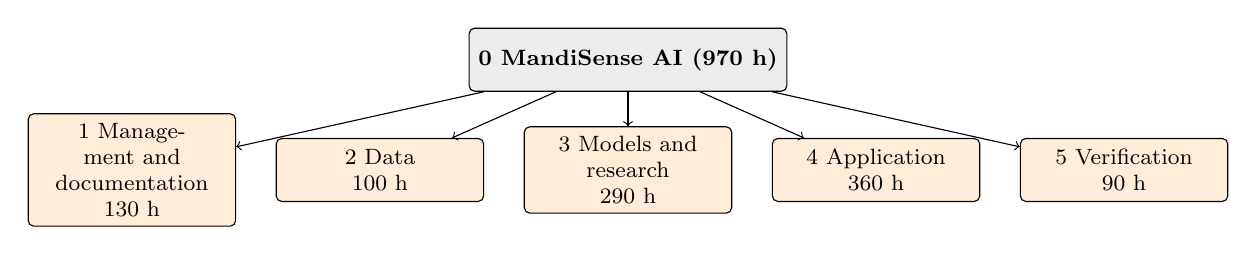
\begin{tikzpicture}[every node/.style={font=\footnotesize}, p/.style={draw, rounded corners=2pt, fill=orange!15, text width=2.4cm, align=center, minimum height=8mm}, c/.style={draw, rounded corners=2pt, fill=blue!6, text width=2.5cm, align=center, minimum height=7mm}, level distance=1.4cm, sibling distance=3.15cm, edge from parent/.style={draw, ->}]
\node[draw, fill=gray!15, rounded corners=2pt, minimum height=8mm] {\textbf{0 MandiSense AI (970 h)}}
  child {node[p] {1 Management and documentation\\130 h}}
  child {node[p] {2 Data\\100 h}}
  child {node[p] {3 Models and research\\290 h}}
  child {node[p] {4 Application\\360 h}}
  child {node[p] {5 Verification\\90 h}};
\end{tikzpicture}
\caption{Level-1 work breakdown structure with estimated hours.}
\label{fig:wbs}
\end{figure}

\begin{table}[!t]
\centering
\caption{Work breakdown with owner and estimated hours (estimates, not logged time)}
\label{tab:wbs}
\small
\begin{tabular}{|l|p{6.2cm}|l|r|}
\hline
\textbf{WBS} & \textbf{Task} & \textbf{Owner} & \textbf{Hours} \\ \hline
\textbf{1} & \textbf{Management and documentation} & & \textbf{130} \\
1.1 & Requirements and literature survey & Shreejith & 40 \\
1.2 & Planning and tracking & Shreejith & 20 \\
1.3 & Final report, appendices, similarity record & Shreejith & 70 \\ \hline
\textbf{2} & \textbf{Data} & & \textbf{100} \\
2.1 & Agmarknet acquisition & Manohara & 20 \\
2.2 & Cleaning, integrity checks, exclusions & Manohara & 40 \\
2.3 & Market panel and observation store & Manohara & 40 \\ \hline
\textbf{3} & \textbf{Models and research} & & \textbf{290} \\
3.1 & Market-choice formulation and engines, floors & Manohara & 90 \\
3.2 & Forecasters and specialist council & Manohara & 60 \\
3.3 & Experiments, statistics, leakage audit & Manohara & 100 \\
3.4 & Shock study and cross-commodity spillover & Manohara & 40 \\ \hline
\textbf{4} & \textbf{Application} & & \textbf{360} \\
4.1 & Backend API & Srijan & 90 \\
4.2 & Farmer web application & Srijan & 90 \\
4.3 & Trader web application & Srijan & 60 \\
4.4 & Decision-intelligence briefs, explanation layer, chatbot & Srijan & 60 \\ \hline
4.5 & Insight features and Telegram digest (API, pages, bot, tests) & Srijan & 60 \\ \hline
\textbf{5} & \textbf{Verification} & & \textbf{90} \\
5.1 & Test plan and validation & Shreejith & 50 \\
5.2 & Integration, pipeline, fresh-clone check & Manohara & 40 \\ \hline
\multicolumn{3}{|r|}{\textbf{Total}} & \textbf{970} \\ \hline
\end{tabular}
\end{table}

\section{Activity Network and Critical Path}
\label{sec:network}

The leaf tasks were grouped into eleven activities (Table~\ref{tab:activities}). Planned durations are in weeks; the network is in Figure~\ref{fig:network}.

\begin{table}[!t]
\centering
\caption{Activities, predecessors and planned durations}
\label{tab:activities}
\small
\begin{tabular}{|c|p{5.6cm}|c|c|c|c|c|c|}
\hline
\textbf{ID} & \textbf{Activity} & \textbf{Pred.} & \textbf{Dur.} & \textbf{ES} & \textbf{EF} & \textbf{LS} & \textbf{Slack} \\ \hline
A & Requirements and literature & --- & 2 & 0 & 2 & 0 & 0 \\ \hline
B & Data acquisition and cleaning & A & 3 & 2 & 5 & 2 & 0 \\ \hline
C & Market-choice formulation, engines & B & 4 & 5 & 9 & 5 & 0 \\ \hline
D & Backend API & A & 4 & 2 & 6 & 7 & 5 \\ \hline
E & Web application (farmer, trader) & D & 5 & 6 & 11 & 11 & 5 \\ \hline
F & Forecasters and council & C & 3 & 9 & 12 & 9 & 0 \\ \hline
G & Experiments, statistics, leakage & C, F & 4 & 12 & 16 & 12 & 0 \\ \hline
H & Decision intelligence, explanation layer, chatbot & D & 3 & 6 & 9 & 13 & 7 \\ \hline
I & Testing and validation & E, G, H & 3 & 16 & 19 & 16 & 0 \\ \hline
J & Integration and reproducibility & I & 2 & 19 & 21 & 19 & 0 \\ \hline
K & Report and documentation & J & 3 & 21 & 24 & 21 & 0 \\ \hline
\end{tabular}
\end{table}

\begin{figure}[!t]
\centering
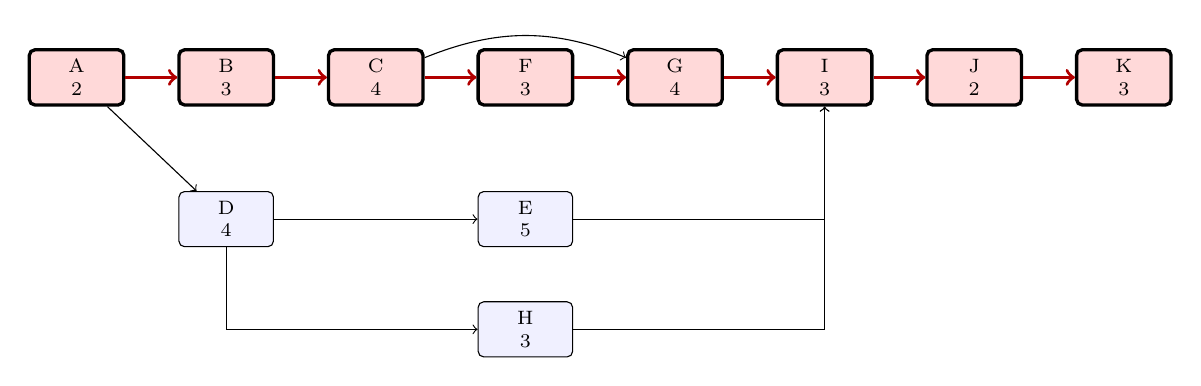
\begin{tikzpicture}[every node/.style={font=\scriptsize}, n/.style={draw, rounded corners=2pt, minimum width=1.2cm, minimum height=7mm, align=center}, cr/.style={n, fill=red!15, very thick}, nc/.style={n, fill=blue!6}]
\node[cr] (A) at (0,0) {A\\2};
\node[cr] (B) at (1.9,0) {B\\3};
\node[cr] (C) at (3.8,0) {C\\4};
\node[cr] (F) at (5.7,0) {F\\3};
\node[cr] (G) at (7.6,0) {G\\4};
\node[cr] (I) at (9.5,0) {I\\3};
\node[cr] (J) at (11.4,0) {J\\2};
\node[cr] (K) at (13.3,0) {K\\3};
\node[nc] (D) at (1.9,-1.8) {D\\4};
\node[nc] (E) at (5.7,-1.8) {E\\5};
\node[nc] (H) at (5.7,-3.2) {H\\3};
\draw[->, very thick, red!70!black] (A)--(B); \draw[->, very thick, red!70!black] (B)--(C); \draw[->, very thick, red!70!black] (C)--(F);
\draw[->, very thick, red!70!black] (F)--(G); \draw[->, very thick, red!70!black] (G)--(I); \draw[->, very thick, red!70!black] (I)--(J); \draw[->, very thick, red!70!black] (J)--(K);
\draw[->] (A)--(D); \draw[->] (D)--(E); \draw[->] (D)|-(H);
\draw[->] (C) to[bend left=22] (G);
\draw[->] (E)-|(I); \draw[->] (H)-|(I);
\end{tikzpicture}
\caption{Activity-on-node network. The critical path A--B--C--F--G--I--J--K is shown in red; durations are in weeks.}
\label{fig:network}
\end{figure}

\noindent\textbf{Worked calculation.} The forward pass gives $EF_K=24$ weeks, which is the planned duration. For the backward pass, $LF_K=24$ and $LS_K=24-3=21$; $LS_J=21-2=19$; $LS_I=19-3=16$; $LS_G=16-4=12$; $LS_F=12-3=9$; $LS_C=\min(LS_F,LS_G)-4=9-4=5$; $LS_B=2$; $LS_A=0$. The path with zero slack is therefore A--B--C--F--G--I--J--K, of length $2+3+4+3+4+3+2+3=24$ weeks. For activity E, $LF_E=LS_I=16$, so $LS_E=16-5=11$ and slack $=LS_E-ES_E=11-6=5$ weeks. For H, $LS_H=16-3=13$ and slack $=13-6=7$. For D, $LF_D=\min(LS_E,LS_H)=\min(11,13)=11$, so $LS_D=7$ and slack $=7-2=5$.

\noindent\textbf{Consequence.} The application work (D, E, H) had slack and the research chain did not. In practice the research chain was reopened late (Section~\ref{sec:risks}), which is why the project overran.

\section{Schedule: Baseline against Actual}
\label{sec:gantt}

The baseline runs 24 weeks from 27 April 2026 (week 0) and was reconstructed from the Phase-1 roadmap. Actual spans come from commit dates (first commit 28 April 2026, last 29 October 2026); the repository shows no activity between 10 June and 28 September, so the bars for E and D show continuous spans that include that gap. Total slip is about 3.3 weeks (14\% over the 24-week baseline). The insight features and the Telegram digest were added after the research results were complete; they are outside the 24-week baseline and add an estimated 60 hours (Table~\ref{tab:wbs}).

\begin{figure}[!t]
\centering
\begin{tikzpicture}[x=0.42cm, y=0.55cm, font=\scriptsize]
\foreach \w in {0,4,...,28} {\draw[gray!40] (\w,0.6) -- (\w,-11.8); \node at (\w,1) {\w};}
\node[anchor=east] at (-0.3,1) {week};
\def\row#1#2#3#4#5#6{\node[anchor=east] at (-0.3,-#1) {#2}; \fill[blue!25] (#3,-#1+0.12) rectangle (#4,-#1+0.42); \fill[orange!85!black] (#5,-#1-0.42) rectangle (#6,-#1-0.12);}
\row{0.5}{A Requirements}{0}{2}{0}{3}
\row{1.7}{B Data}{2}{5}{3}{24}
\row{2.9}{C Market choice}{5}{9}{6}{26}
\row{4.1}{D Backend API}{2}{6}{1}{23}
\row{5.3}{E Web application}{6}{11}{6}{24}
\row{6.5}{F Forecasters}{9}{12}{22}{26}
\row{7.7}{G Experiments}{12}{16}{24}{27}
\row{8.9}{H Explanation layer}{6}{9}{22}{24}
\row{10.1}{I Testing}{16}{19}{22}{27}
\row{11.3}{J Integration}{19}{21}{25}{27}
\row{12.5}{K Report}{21}{24}{25}{27.3}
\foreach \m/\l in {3/M1,6/M2,22/M3,26/M4,27.3/M5} {\node[diamond, fill=red!70, inner sep=1.2pt] at (\m,-13.6) {}; \node[below] at (\m,-13.8) {\l};}
\fill[blue!25] (0,-15.2) rectangle (1,-15); \node[anchor=west] at (1.2,-15.1) {baseline};
\fill[orange!85!black] (6,-15.2) rectangle (7,-15); \node[anchor=west] at (7.2,-15.1) {actual};
\end{tikzpicture}
\caption{Baseline (blue) against actual (orange) schedule. Milestones: M1 requirements and literature complete (week 3); M2 first deployed prototype, 9 June (week 6); M3 farmer feature suite, 30 September (week 22); M4 research results and release, 29 October (week 26); M5 final report (week 27).}
\label{fig:gantt}
\end{figure}

\begin{table}[!t]
\centering
\caption{Schedule variance by activity (weeks from 27 April 2026; actual spans from commits)}
\label{tab:variance}
\small
\begin{tabular}{|c|c|c|c|c|p{4.6cm}|}
\hline
\textbf{ID} & \textbf{Baseline} & \textbf{Actual} & \textbf{Finish slip} & \textbf{On critical path} & \textbf{Reason} \\ \hline
A & 0--2 & 0--3 & +1 & yes & Scope clarified after first review \\ \hline
B & 2--5 & 3--24 & +19 & yes & Data reopened (Sec.~\ref{sec:risks}, R1) \\ \hline
C & 5--9 & 6--26 & +17 & yes & Re-specified on real labels \\ \hline
D & 2--6 & 1--23 & +17 & no & Slack absorbed it \\ \hline
E & 6--11 & 6--24 & +13 & no & Farmer suite added in September \\ \hline
G & 12--16 & 24--27 & +11 & yes & Waited for rebuilt panel \\ \hline
K & 21--24 & 25--27.3 & +3.3 & yes & Project finish \\ \hline
\end{tabular}
\end{table}

\section{Responsibility Assignment Matrix}
\label{sec:ram}

Table~\ref{tab:ram} assigns each work package using R (responsible), A (accountable), C (consulted), I (informed). The guide is accountable for approval of each package. The split matches the owners in Table~\ref{tab:wbs}.

\begin{table}[!t]
\centering
\caption{RACI matrix by work package}
\label{tab:ram}
\small
\begin{tabular}{|l|c|c|c|c|}
\hline
\textbf{Package} & \textbf{Manohara} & \textbf{Srijan} & \textbf{Shreejith} & \textbf{Guide} \\ \hline
1 Management and documentation & C & C & R & A \\ \hline
2 Data & R & I & C & A \\ \hline
3 Models and research & R & C & C & A \\ \hline
4 Application & C & R & I & A \\ \hline
5 Verification & R (5.2) & C & R (5.1) & A \\ \hline
\end{tabular}
\end{table}

Hours by owner follow from Table~\ref{tab:wbs}: Manohara 430, Srijan 360, Shreejith 180, a total of 970.

\noindent\textbf{Contribution record.} The repository's commit history (\texttt{docs/CONTRIBUTIONS.md}) shows 64 commits by Manohara, 1 by Srijan and none by Shreejith. The owners above are the team's agreed split; the history does not corroborate the work of the second and third members, and work done on other machines would not appear in it.

\section{Risk Register}
\label{sec:risks}

\begin{table}[!t]
\centering
\caption{Risk register. Probability (P) and impact (I) on a 1--5 scale; exposure E $=$ P$\times$I. Status shows whether the risk occurred.}
\label{tab:risks}
\small
\begin{tabular}{|c|p{4.1cm}|c|c|c|p{4.0cm}|p{2.7cm}|}
\hline
\textbf{ID} & \textbf{Risk} & \textbf{P} & \textbf{I} & \textbf{E} & \textbf{Mitigation / response} & \textbf{Status} \\ \hline
R1 & Source data not real: the first dataset in the repository was synthetic & 3 & 5 & 15 & Re-acquired Agmarknet exports; integrity check between exports; synthetic removed & \textbf{Occurred} \\ \hline
R2 & Look-ahead leakage in features or evaluation & 4 & 5 & 20 & Leakage unit tests; causal protocol & \textbf{Occurred}; two whole-series-centred features, caught by test \\ \hline
R3 & Hard deletion of records breaks trader pages & 3 & 3 & 9 & Soft delete and re-seeding & \textbf{Occurred} \\ \hline
R4 & Dependency break (NumPy upgrade) & 3 & 3 & 9 & Pinned NumPy 1.26.4, regenerated lock file & \textbf{Occurred} \\ \hline
R5 & LLM API rate limit (8,000 tokens per minute) & 4 & 2 & 8 & Throttling; small evaluation set & \textbf{Occurred} \\ \hline
R6 & Uneven contribution within the team & 3 & 4 & 12 & Contribution record; owner split; guide review & Open \\ \hline
R7 & Public deployment not verified end to end & 3 & 3 & 9 & Docker and Render files provided; not tested live & Open \\ \hline
R8 & No field trial with farmers & 4 & 3 & 12 & Stated as limitation; survey instrument ready & Open \\ \hline
R9 & Agmarknet changes export format & 2 & 4 & 8 & Loader rejects unexpected units and keys & Not occurred \\ \hline
R10 & Stale development servers answered with old code while new features were tested & 3 & 2 & 6 & Restart after every change; smoke test lists every new endpoint and page & \textbf{Occurred} \\ \hline
\end{tabular}
\end{table}

\noindent\textbf{Risk R1 in detail.} The most costly event was the discovery that the first dataset in the repository was synthetic and that results derived from it had no meaning. It was found late in the project. The response was to discard it, rebuild the panel from the portal exports, and re-run every experiment. This is the main cause of the slip in B, C and G (Table~\ref{tab:variance}), and it is why critical-path activities, not slack activities, absorbed the delay.

\section{Resources and Cost}
\label{sec:cost}

\begin{table}[!t]
\centering
\caption{Resource and cost summary. Labour is notional at Rs 200 per hour; no cash was paid for it.}
\label{tab:cost}
\small
\begin{tabular}{|l|p{6.2cm}|r|r|}
\hline
\textbf{Resource} & \textbf{Basis} & \textbf{Units} & \textbf{Cost (Rs)} \\ \hline
Labour -- Manohara & 430 h at Rs 200 & 430 & 86,000 \\ \hline
Labour -- Srijan & 360 h at Rs 200 & 360 & 72,000 \\ \hline
Labour -- Shreejith & 180 h at Rs 200 & 180 & 36,000 \\ \hline
Compute & Team laptop (Table~\ref{tab:hardware-req}), already owned & --- & 0 \\ \hline
Data & Agmarknet public portal & --- & 0 \\ \hline
Language model API & Free tier of the provider & --- & 0 \\ \hline
Hosting & Free tiers (deployment not verified) & --- & 0 \\ \hline
\textbf{Total notional} & & 970 & \textbf{1,94,000} \\ \hline
\textbf{Cash spent} & & & \textbf{0} \\ \hline
\end{tabular}
\end{table}

Labour totals match the hours in Table~\ref{tab:wbs}. No tool or service with a licence fee was used.
